\documentclass{sigchi}

% Use this command to override the default ACM copyright statement (e.g. for preprints). 
% Consult the conference website for the camera-ready copyright statement.


%% EXAMPLE BEGIN -- HOW TO OVERRIDE THE DEFAULT COPYRIGHT STRIP -- (July 22, 2013 - Paul Baumann)
% \toappear{Permission to make digital or hard copies of all or part of this work for personal or classroom use is 	granted without fee provided that copies are not made or distributed for profit or commercial advantage and that copies bear this notice and the full citation on the first page. Copyrights for components of this work owned by others than ACM must be honored. Abstracting with credit is permitted. To copy otherwise, or republish, to post on servers or to redistribute to lists, requires prior specific permission and/or a fee. Request permissions from permissions@acm.org. \\
% {\emph{CHI'14}}, April 26--May 1, 2014, Toronto, Canada. \\
% Copyright \copyright~2014 ACM ISBN/14/04...\$15.00. \\
% DOI string from ACM form confirmation}
%% EXAMPLE END -- HOW TO OVERRIDE THE DEFAULT COPYRIGHT STRIP -- (July 22, 2013 - Paul Baumann)


% Arabic page numbers for submission. 
% Remove this line to eliminate page numbers for the camera ready copy
% \pagenumbering{arabic}


% Load basic packages
\usepackage{balance}  % to better equalize the last page
\usepackage{graphics} % for EPS, load graphicx instead
\usepackage{times}    % comment if you want LaTeX's default font
\usepackage{url}      % llt: nicely formatted URLs
\usepackage{csquotes}
\usepackage{textcomp}

% llt: Define a global style for URLs, rather that the default one
\makeatletter
\def\url@leostyle{%
  \@ifundefined{selectfont}{\def\UrlFont{\sf}}{\def\UrlFont{\small\bf\ttfamily}}}
\makeatother
\urlstyle{leo}


% To make various LaTeX processors do the right thing with page size.
\def\pprw{8.5in}
\def\pprh{11in}
\special{papersize=\pprw,\pprh}
\setlength{\paperwidth}{\pprw}
\setlength{\paperheight}{\pprh}
\setlength{\pdfpagewidth}{\pprw}
\setlength{\pdfpageheight}{\pprh}

% Make sure hyperref comes last of your loaded packages, 
% to give it a fighting chance of not being over-written, 
% since its job is to redefine many LaTeX commands.
\usepackage[pdftex]{hyperref}
\hypersetup{
pdftitle={CS2300 Personal Informatics final paper},
pdfauthor={LaTeX},
pdfkeywords={SIGCHI, proceedings, archival format},
bookmarksnumbered,
pdfstartview={FitH},
colorlinks,
citecolor=black,
filecolor=black,
linkcolor=black,
urlcolor=black,
breaklinks=true,
}

% create a shortcut to typeset table headings
\newcommand\tabhead[1]{\small\textbf{#1}}


% End of preamble. Here it comes the document.
\begin{document}

\title{CS2300 Personal Informatics final paper}

\numberofauthors{5}
\author{
  \alignauthor Karthik Desingh\\
    \email{$karthik$\textunderscore$desingh@brown.edu$}    
  \alignauthor Elyse McManus\\
    \email{$elyse$\textunderscore$mcmanus@brown.edu$}       
  \alignauthor Vitor Oliveira\\
    \email{$vitor$\textunderscore$oliveira@brown.edu$}       
  \alignauthor Quinn Li O'shea\\
    \email{$quinn$\textunderscore$li$\textunderscore$oshea@brown.edu$}       
  \alignauthor Lixiang Zhang\\
    \email{$lixiang$\textunderscore$zhang@brown.edu$}       
}

\maketitle

\begin{abstract}
Personal informatics experimentation is a growing area of research used for self-exploration. There are many ways to run personal informatics experiments, some more scientifically rigorous than others, and there is no template for how these experiments should be constructed. In this study, we had 21 students in a graduate level computer science course run a personal informatics experiment on themselves for a month, tracking at least two variables to see if there would be any significant changes. These students had a brief overview of standard research practices and some, but not all, had statistical backgrounds to better analyze their data. Each student ran their experiment differently, in a way that fit in with their day to day life. At the end of the experiment, a variety of statistical tests were used to evaluate the data. 
\\
We find that personal informatics experiments are best left up to individuals to tweak and tailor to meet their demands. Users should design these studies specific to their needs. Since everyone lives differently, there is no set formula for how these kinds of studies should be run. In designing their experiments, we found that it was helpful to have a long enough time to run the experiment; use technologies that automatically track variables; and have some sort of background in statistics to find statistically meaningful results. 
\end{abstract}
%
%\keywords{
%	Guides; instructions; author's kit; conference publications;
%	keywords should be separated by a semi-colon. \newline
%	\textcolor{red}{Optional section to be included in your final version, 
%  but strongly encouraged.}
%}

%\category{H.5.m.}{Information Interfaces and Presentation (e.g. HCI)}{Miscellaneous}
%
%See: \url{http://www.acm.org/about/class/1998/}
%for more information and the full list of ACM classifiers
%and descriptors. \newline
%\textcolor{red}{Optional section to be included in your final version, 
%but strongly encouraged. On the submission page only the classifiers’ 
%letter-number combination will need to be entered.}

\section{Introduction}
We have yet to encounter research on individuals conducting their own personal informatics experiments. In this paper we plan to fill in this gap in the field of personal tracking by providing an overview of twenty-one individuals' personal informatics experiments, each of whom were enrolled in the Human Computer Interaction Seminar at Brown University. Each experimenter was instructed to design their own experiment spanning a month and analyze their results upon completion. Every student had to choose at least one independent variable, two dependent variables, formulate at least two related hypotheses, and design an experiment to test their hypotheses. No one in the class was allowed to have the same set of variables and hypotheses as another classmate.  
 
All twenty-one students employed various methods to track their variables throughout their respective experiments.  The class was made up of twelve male and nine female students, representing every level of education offered at Brown University besides freshmen.  There were two sophomores, two juniors, four seniors, four Master’s students, six PhD students, and one unknown. (The one unknown is a result of student backgrounds being gained through a voluntary survey we sent out post-experiment completion. One member of the seminar did not fill out our survey.)
 
Every member of the class was given the same set of directions. These directions instructed that they could track any combination of independent and dependent variables, as long as there was a hypothesis that could be tested and that the data regarding the variables could be analyzed. Across the twenty-one studies, commonalities in the various aspects of the process of the experiment were observed, including dependent variables, confounding factors, and statistical results. While there were several distinct dependent variables, we explore questions such as: Why were some of the most common ones studied by almost everyone in the class? Why were so many users' results, post analysis, considered insufficient to make any definite claims? We believe that by examining these twenty-one reports on personalized experiments, we will be able to answer these questions and gain insight pertaining to the motivations behind tracking certain variables, factors necessary for successful personal-informatics tracking, and other valuable aspects of completing personal informatics experiments.
\section{Related work}
TODO
\section{Technology}
A wide range of technologies and methods were used to collect data for this assignment. All of the tracking technologies can be grouped into three categories: devices, mobile apps, and desktop software. Fig.\ref{fig:technology} shows the number of students who used technologies in the given categories. 

\begin{figure}[!t]\centering
	%\begin{wrapfigure}{o}{\textwidth}\centering
	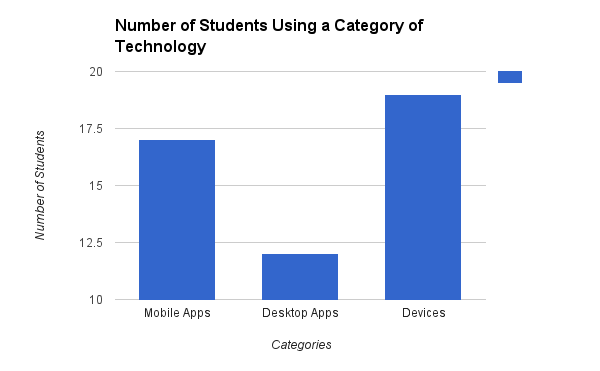
\includegraphics[width=1.0\columnwidth]{images/technology_chart.png}
	\caption{\footnotesize Distribution of technologies used by students\label{fig:technology} 
	}%\end{wrapfigure}
\end{figure}
%

\subsection{Devices}
    The class used numerous devices to keep track of their data for the assignment. Many students used standard devices and manually logged their data into a spreadsheet of some sort. To measure weight, students used a regular scale and logged the data in a spreadsheet. One student used a timer to count their pulse to get their heart rate. Other students used the reportings found on treadmills. 
    Other students used devices that kept track of the data for them. Several students monitored their sleeping patterns using devices like the Garmin Vivofit and the FitBit. These devices track the time it takes to fall asleep, how long the user is sleeping, how many times the user wakes up during the night, and in some cases how long the user is in deep sleep, REM sleep, or light sleep. The data is then uploaded and displayed in some sort of dashboard, usually accessible online. These devices are typically worn on the user as they sleep. The FitBit, for example, is worn on the wrist during sleep. One user used the Garmin  nüvi to keep track of their location with the GPS feature. 

\subsection{Mobile apps} 
    Many users opted to use mobile apps to keep track of their data. Out of the 17 mobile apps used, 13 were iPhone apps and 4 were Android apps. Self reporting apps like Reporter and Lume were used to collect data about the user throughout the day. These apps logged qualitative data about daily aspects of life such as mood, energy, and thoughts. 
    Some of the apps tracked user data automatically. Moment tracked mobile activity on iDevices logging how long a user spent on their phone or iPad throughout the day. Several users used sleep apps similar to the sleep devices mentioned above that tracked various quantitative aspects of sleep. These apps were the Sleep As Android app and the iPhone Sleep Cycle app. Users put their phones on their beds as they slept and the apps tracked things like movement and such. The Galaxy S-Health app was also used to track number of steps and log various health-related aspects of the user’s day to day activities like food intake and stress level.
    
\subsection{Desktop software} 
    Many participants also used desktop software to track their variables. Many users would take a measurement with a device or apparatus that did not automatically record the data and manually log or correct the data themselves, as mentioned above in the devices section. In relation to the FitBit device mentioned above, the FitBit dashboard was used to view data and in some cases manually log data when necessary. Spreadsheets, both Microsoft\textquotesingle s Excel and Google Spreadsheets, were also used to manually log data that was either collected using the devices mentioned above or other data that was not captured using a device. One example of this would be the user that logged the ph of their saliva by using ph test strips and writing their ph level into a spreadsheet. 
    Other students used apps that automatically tracked certain data. Several used apps that monitored their computer usage like TimeStats and Rescue time. These apps kept track of the amount of time spent on certain apps or websites during computer or browser usage. Weather.com was also used to retroactively look up data about the weather and temperatures for the day. Online banking apps were also used to keep track of spending.
\section{Experimental Design}

While performing various experiments, users had to choose an experimental design that would deliver the best results without introducing biases. During an experiment, especially one running for 28 days, experimental design is extremely important. During an experiment a user changes an independent variable in order to observe how it affects one or more dependent variables. In order to notice any and garner the most and best effects, the user must come up with a way to lay out how their experiment will run, thinking in advance of any factors that might affect their experiment and attempt to control for that. The 21 participants in this study chose various experimental designs but most can be broken down into two different designs. 
    The first design is involves randomization. Participants that chose this experimental design would flip a coin or find a random way to either perform or not perform their independent variable, such as running that day or not, or showering before sleep or not. This method limits environmental and temporal biases that might otherwise exist. Some examples of these biases include differences in behavior during weekdays versus weekends or even external circumstances such as having a busy day or week due to class projects, exams, homework, etc. Randomization ignores these factors because a user might be busy two days in a row but perhaps one day the coin flips \enquote*{heads} while the other day it flips \enquote*{tails} controlling for any personal biases. 
    The other common experimental design was the AB\textunderscore\textunderscore  design and variations on that. These variations included ABA, AB, ABCD, ABA, ABAC. In this experimental design, users perform a certain behavior equally for a period of time (A) then switch to a different behavior for another period of time (B), and so on, each letter delineating a difference in the way they perform their independent variable. This experimental design fits some experiments better than say, randomization, because some effects might take longer to come into effect than others and so running it for a longer period of time (versus just one day) might affect the data. This experimental design also allows for participants to run experiments where they try a behavior, go to a different behavior (including the complete lack of that behavior), and finally return to the original behavior in order to analyze different effects. 
    Overall, users were careful in designing their experiments so that they could introduce the least amount of biases into their data. Unfortunately for some, especially those running the variations of AB\textunderscore\textunderscore  experimental design, temporal biases were introduced especially due to the last week of the experiment coinciding with spring break whereas those running their experiment through randomization did not have as much of a problem with this confounding factor which we touch upon later in the paper. 

\section{Dependent Variables}
Participants in this project have been given the freedom to choose their own independent and dependent variables. This resulted in wide variety of variables to be tracked as there were varying interests and varying behavioral changes that participants wanted to experiment on. Below is the list of dependent variables that 21 participants tracked in this project. Please note that some of the variables have been grouped into a particular category. For examples the \enquote{Exercise} in the Fig.\ref{fig:variables} includes variables like \enquote{Pacing your run}  , \enquote{Swimming} and \enquote{Exercise occurrences}.

\begin{figure}[!t]\centering
%\begin{wrapfigure}{o}{\textwidth}\centering
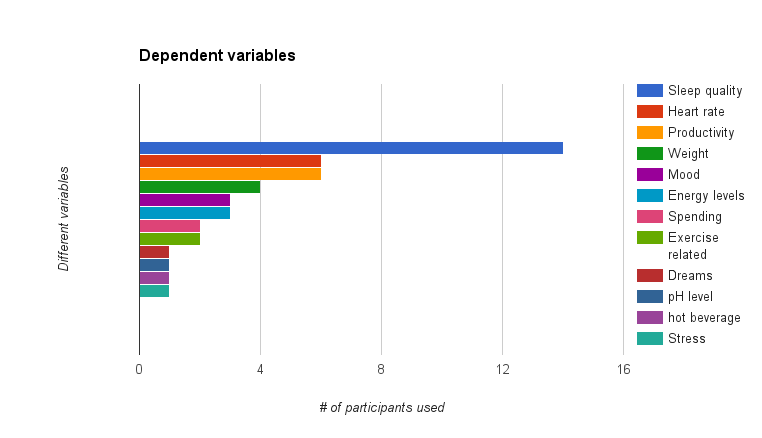
\includegraphics[width=1.0\columnwidth]{images/dependent_variables.png}
\caption{\footnotesize Dependent variables tracked in the class study \label{fig:variables} 
}%\end{wrapfigure}
\end{figure}
%
It is very evident from Fig.\ref{fig:variables} that many participants felt necessary to track their sleep quality. Since the participant group are students of top tier college, it makes sense that sleep is something they care about in their lifestyle amidst loads of deadlines and activities. Also one can note from the previous section that the most of the devices participants used gives sleep quality as their main feature. Hence with sleep quality being the most important factor the participant group cares and it being the most easy variable that can be tracked using the devices, it is no surprise that 14 participants tracked this variable. 

After Sleep quality, Heart rate is another feature that wearable devices care to track about. With increasing heart diseases globally, this is one of most used metric to show if a person is healthy. Hence Heart rate is a variable that participants had easy access to and wanted to know the changes it had on their behavioral changes.

Productivity is a variable that participant group cared about as it is something that they want to improve on a daily basis in one form or the other. Factors that determine productivity varies from individual to individual and tracking devices fail to capture this personalized subjective variable. Hence participants came up with interesting self reporting techniques that will be discussed in detail in section.

Weight is another variable that participant group cared to track with respect to their behavior changes. Weight has been traditionally something that people cared in terms of that affecting their appearance and also it being a good metric to judge your health status. So it came out to be one of the obvious variables that participant group chose in this experiment. 

Though there are other interesting variables people tracked during the experiment. this paper will focus on the top 4 variables and discuss insights and observations from the participants in detail.

\begin{figure*}[!t]\centering
%\begin{wrapfigure}{o}{\textwidth}\centering
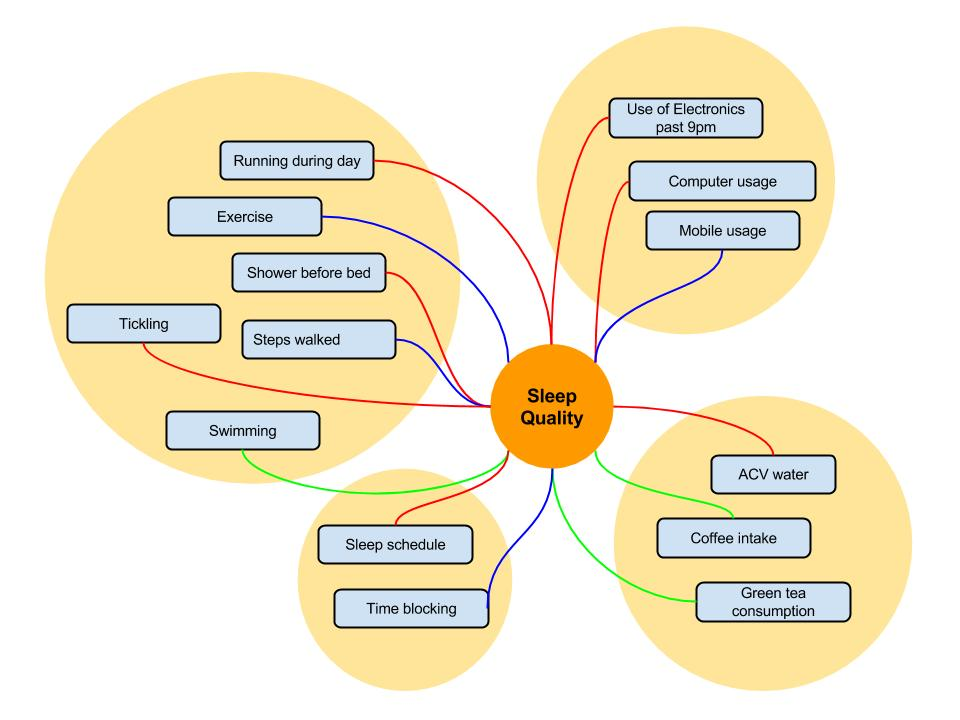
\includegraphics[width=0.47\textwidth]{images/Sleep_quality.jpg}
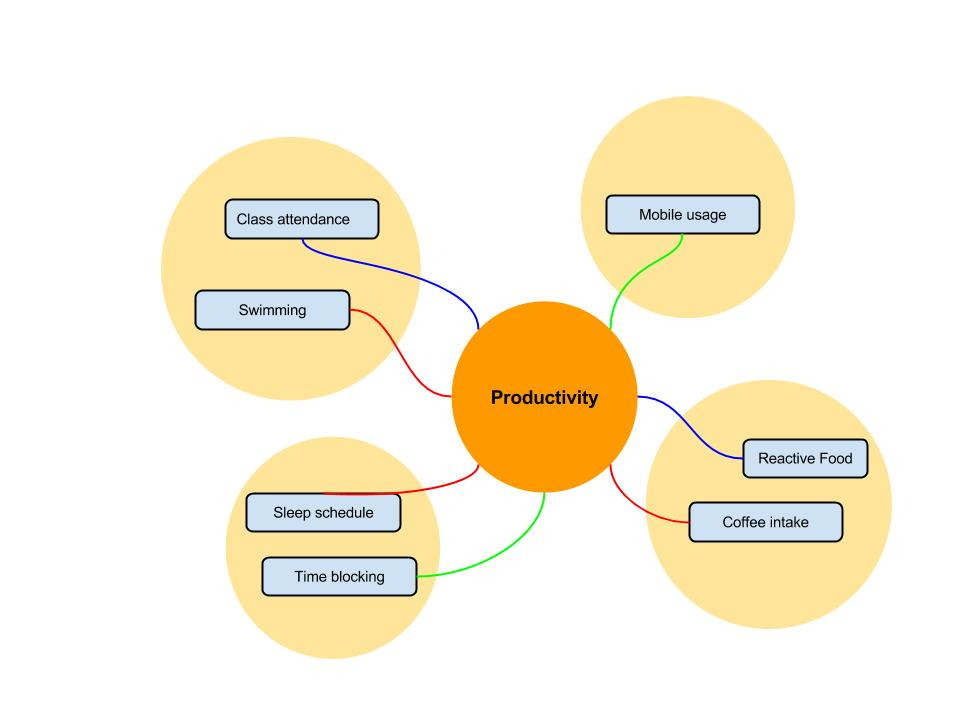
\includegraphics[width=0.47\textwidth]{images/Productivity.jpg}
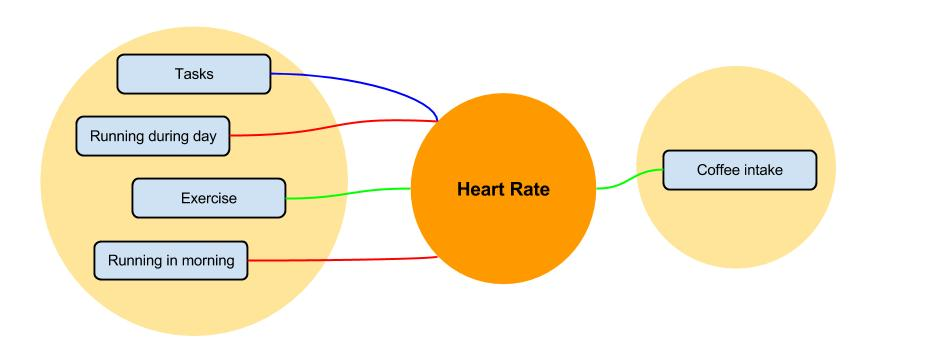
\includegraphics[width=0.47\textwidth]{images/Heart_rate.jpg}
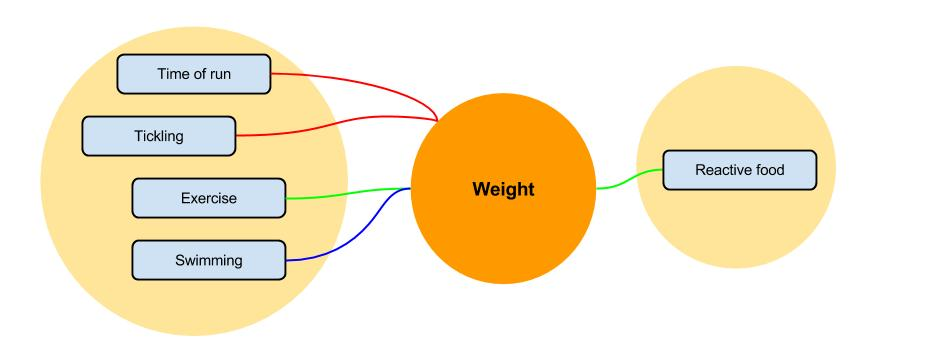
\includegraphics[width=0.47\textwidth]{images/Weight.jpg}
\caption{\footnotesize Dependent variables and the independent variables that were related to it by the participants \label{fig:dependentvsindependent} 
}%\end{wrapfigure}
\end{figure*}

\subsection{Sleep quality}
For tracking sleep, participants used various applications and devices from Sleep As Android to FitBit which kept track of the amount of time people were in various levels of sleep (light, deep, R.E.M.) and how many times they woke up during the night. Devices have various approaches to measuring sleep quality. Mobile apps use ambient noise and movements in the bed to measure the sleep quality. Some wearable devices use body movements and others use a pulse sensor to measure sleep quality. The quality of the measurements is directly proportional to the cost of the device and hence the reported sleep quality measurements are approximations. 

It is interesting to see what each participant\textquotesingle s hypothesis were and the independent variables that they hypothesized to affect sleep quality. Below figure shows all the independent variables that were reported directly related to sleep quality by the participants. The independent variables have been clustered into categories \enquote{usage of devices}, \enquote{activities}, \enquote{schedule changes} and \enquote{consumption of drinks}. The green edges indicates that these variables affect sleep quality. The red edge indicates that these variables do not have an effect on the sleep quality. The blue edge indicates that the experiments on these variables have not had any conclusion due to less data points.

For the most part, least number (3) of variables seem to have affected sleep. Most of all the hypotheses (7) have been rejected by the participants. Significant number of hypotheses were inconclusive (4). 

A common observation from the reports of the participants is that their hypothetical behavior that affects the sleep quality is not always true. For example, activities (except swimming) and device usage had no effect on the sleep quality as observed by the participants. Also one would certainly assume that a better schedule of the day will improve the sleep quality, but its been proven otherwise in this study. These are some interesting insights about the factors affecting sleep quality. 

But one must note that, all these are conclusions highly biased to the individuals and their tracking methods. If every participant used a single common tracking mechanism to track the sleep quality, then it is easy to conclude in general that a particular behavior either improves or worsens the sleep quality. However with constraint on the number of days and experimental design one can adopt, some of these conclusions have given insights of what variables one might want to consider when they are tracking their sleep quality.

Some interesting observations by the participants are: a) one participant had trouble falling asleep once they restricted their use of electronics, so they started reading to fill the time; b) one participant woke up more according to their findings; c) one of the user had seen improvement of 29 percent in the sleep quality when they swam in the night between 9-10.30 pm. 

Others did not come to a conclusion because they felt the the variable was not properly tracked, for example, mobile devices were not as reliable in tracking sleep in comparison to wearable device. Some of the wearable devices track the motion of the hand to measure the sleep time and that could also be noisy and not accurate. So it may be the case that the data points has to be definitely more than 28 days to come to any conclusion on this regard. In addition to this the users are supposed to design their experiment in AB, ABA, ABAC etc format so they have less data points to the significant change they are tracking and I feel that the \enquote{Jet lag} pointed by one of the participant plays a significant role in producing the transition data.

\subsection{Productivity}


Productivity is a subjective variable and in order to quantify, participants used metrics created based on the completeness of anticipated tasks, \enquote{productivity pulse} through RescueTime software, 1-10 scale based on time, 1-7 based on concentration intensity. Some of the apps and plugins used were RescueTime Plugin  and TimeStats Plugin.

Fig.\ref{fig:variables} shows how the independent that variables were related to the Productivity and its outcome at the end of the experiment.

As shown above, except for \enquote{Mobile usage} and \enquote{Time blocking}, all the other independent variables either didn’t have any impact on the productivity or their data points were not enough to conclude any claims.

As far as tracking productivity went, this was one of the most subjective processes.  There is no set metric for productivity nor were there any concrete ways in tracking it.  Across the different studies, productivity was in most cases a self reported process of doing work, through which each student employed some metric to express daily productivity.  This seems acceptable, as every person works differently, encounters personal setbacks and ranges in their times of productivity (whether it\textquotesingle s failing to complete a task or taking too long on a task or getting distracted) and presumably, their chosen methods of data collection and analysis were the ones that fit their perceptions of productivity best.  A common issue encountered with the trackers of productivity was spring break.  Unlike with an action or measurable effects (such as heart rate or weight), productivity is very dependent upon the status of the experimenter\textquotesingle s life.  As spring break arrived, the nature of the work needed to be done changes along with students schedules, rendering parts of time either harder to analyze or irrelevant to the study.  There were mixed results in the effects of different variables\textquotesingle  effects on productivity.  One user found the method of time blocking to be instrumental in significantly increasing their productivity (20-40), while independent variables such as swimming or a fixed sleep schedule did not produce statistically significant changes in productivity.  Class attendance had a significant correlation with productivity and data was just shy of being able to statistically prove it increased the experimenter\textquotesingle s productivity. 

Most importantly defining what is productive is first step in this experiment as experienced by the participants. It needs to be decided what counts as being productive for themselves. Is doing homework productive? Is cooking lunch or checking and answering emails productive? There are various layers and it\textquotesingle s difficult to understand what really is productive to you. Perhaps going to bed instead of staring at that math problem for three hours is more productive. After deciding what constitutes as productive to the user, perhaps they must also decide how intense the work is and how that might affect your data as one user pointed out. Overall, productivity is difficult to keep track of because it\textquotesingle s difficult to quantify an hour of doing mindless work to thirty minutes of intense focused problem solving. 

One common tracking mechanism people had was to self report their activities. Some tools that has helped are reminders from apps like Reporter with some questionnaires about what they did the previous hour? How would they rate their productivity? and so on. Hence there may be significant roles these apps can play to track the productivity. Also tools on desktop to track the amount of time you were on a particular website can in turn give you the details of how many hours have you spent distracted. This also helps the user at the end of the day know how much time he has spend not working on the activity he has to focus on. So there are many tools that can track various aspects of productivity and in consensus with each other based on the logged data can precisely tell the productivity in a day. This is something one could focus to improve upon in Personal informatics domain.

\subsection{Heart rate}
Heart rate is measured either using a wearable tracking device that has special sensors or physically by recording the pulse of a hand. Participants used both these methods in their tracking experiment. 
Fig.\ref{fig:variables} shows how the independent variables were related to the Heart rate and its outcome at the end of the experiment.

Exercise and Coffee intake has an impact on the heart rate. One of the participant made an interesting observation that Coffee intake increases the heart rate immediately after the consumption. Activities overall doesn\textquotesingle t improve the heart rate. Running in different time of the day doesn\textquotesingle t have any impact on the overall heart rate in a day. Participants are in age group of early and mid 20s and so there was no abnormal observations that were made. 

\subsection{Weight}

This being a physical measurement, everyone used the standard scale. Below is the graph show how the independent variables were related to the Weight and its outcome at the end of the experiment.
It can be noticed from above graph that except \enquote{Exercise} and \enquote{Reactive food} non other independent variables had an impact on weight. \enquote{Swimming} didn’t have significant effect on the weight and hence it was declared inconclusive. Overall weight as everyone knows is directly dependent on the food intake and the exercise. Weight is one of the most common factors that people would like to consider since being too fat contributes to hypertension, diabetes and some other diseases while being too skinny may cause to lose self-confidence. 

Some important observations are: a) One of the user showed that there is weight gain once he switched to post- 6PM runs; b) One user noticed that the weight measured in the morning is significantly lower compared to the weight of the body in the night. But none of the experiments have been super conclusive. Tracking the weight is not a noisy/uncertain like other variables we discussed in this section, but an increased duration of the study might have given more conclusive insights.


\section{Independent Variables}

This section presents the chosen independent variables from our 21 self trackers. The dataset spans a wide variety of different variables. For instance, some people track their dependent variables such as sleep quality and productivity and how these are affected by the amount of time spent doing physical activities such as swimming, running and weightlifting. We categorize all these relevant activities into “exercise”. Similarly, other people track their dependent variables such as weight and productivity by measuring the intake of a certain drink such as coffee or tea. We also categorize these independent variables into “beverage intake”. By contrast, some independent variables were unique to some participants in which case we discuss them together in one subsection. By categorizing the different independent variables in this manner, this paper focuses on five main categories which range from Exercise, beverage intake, use of electronic devices, weather conditions, and miscellaneous. This section first demonstrates a chart in the Fig.\ref{fig:chart} followed by the detailed descriptions of each category. 

\begin{figure}[!t]\centering
%\begin{wrapfigure}{o}{\textwidth}\centering
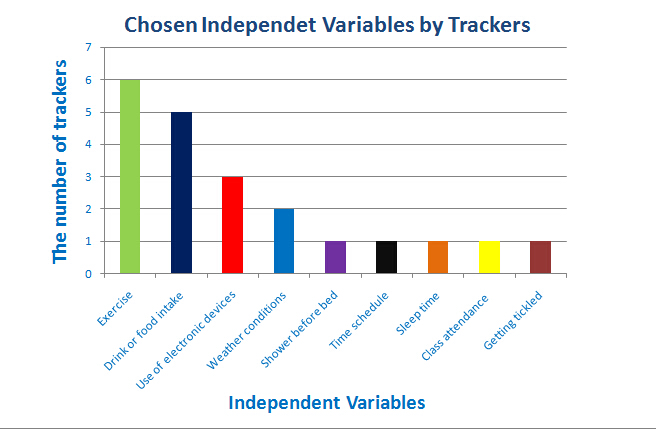
\includegraphics[width=1.0\columnwidth]{images/independent_variables.jpg}
\caption{\footnotesize Independent Variables studied by the participants \label{fig:chart} 
}%\end{wrapfigure}
\end{figure}

Exercise:
Most people are insecure about their body shape. Some would like to build up muscles while others may want to lose or maintain weight. Nowadays, exercise has become one of the most popular activities in people's’ lives. Users often used exercise as an independent variable. It was evaluated in terms of its effects on different dependent variables, including but not limited to all three of the most common dependent variables discussed in this paper. There were reported variations in duration, occurrence, scheduling, and types of exercise as part of experiments’ designs. Exercise is a general term which includes a variety of activities. Of our 21 self trackers, three chose running, one chose swimming, one focused on steps walked per day, and finally one weight lifted as their independent variable. Therefore, “exercise” is one of the most common independent variables being chosen in six out of our 21-participant repository reports.
 
Beverage Intake:
A new study presented at the American Academy of Neurology's 67th Annual Meeting in Washington, DC, suggests yet another potential health benefit of coffee consumption: it could reduce the risk of multiple sclerosis. People are curious about the effects of different beverages on personal health and behavior. Four self trackers chose beverage intake as their independent variables to test out their dependent variables ranging from mood, productivity, pH level, well being, sleep quality and weight gain/loss. The drinks that our trackers used include coffee, green tea, cider apple vinegar water and beer. In this paper, we looked at the relationship between a certain type of drink consumption/intake and overall mortality or productivity.
 
Use of electronic devices:
In the 21st century people are spending more and more time on their electronic devices;Tasks can be easily accomplished using computers and social media connection on apps like Facebook and Twitter are becoming increasingly popular. However, basking in the blue glow of iPads, smartphones and other electronic devices before bedtime could be disrupting sleep patterns more profoundly than we realize, and even affecting our long-term health, according to a new study published Monday in the Proceedings of the National Academy of Sciences. One of our trackers chose the use of electronic devices after 9PM as an independent variable to test out sleep quality and the effect on dreams. And another tracker chose the usage of computer during the day to see how the time spent on the computer affects sleep quality. Similarly, one tracker wants to see how productivity is affected by using cell phone over a certain amount of time.
 
Weather conditions:
As most of the nation suffers through some of the hottest or coldest temperatures on record in summer or winter, people are asking the question of how exactly weather impact our mood? For instance, how does hot weather affect our mood? Does it make us more aggressive or even more violent? Does rain make us sad? Do cold temperatures make us feel more like wanting to hunker down, hibernate, and isolate ourselves from others? So in our 28-day experiment, one of our trackers choose mean of daily temperature as independent variable to identify laziness and the total millimeters of hot beverage intake. Another tracker uses weather conditions (daily temperature, the amount of precipitation and wind speed) to find out how these conditions affect the exercise (exercise types, exercise occurrence and duration of exercise).
Miscellaneous:
Considering the fact that some independent variable is used only by one tracker, these independent variables are not common ones that people use to determine their hypotheses. One tracker is interested in seeing how sleep quality and heart rate are affected by taking a shower before bed. One tracker uses time schedule to test out mood, sleep quality and productivity. One tracker also tries to find out what is the perfect time to go to bed in order to produce the best sleep quality. Additionally, there are two interesting cases where one tracker evaluates mood, sleep quality and weight loss by getting tickled with a hypothesis that getting tickled has positive effect on all those dependent variables and where one tracker identifies how productivity and money spent online are affected by class attendance. 

This paper mainly focuses on the first four categories in that those independent variables are utilized by most of our trackers. Additionally, this statistics seems more likely to be able to be applied to the broader general population as well. This paper does not try to include as many as independent variables but to narrow down to concrete ones and see how dependent variables are affected by these popular independent variables. 

\section{Behavioural Changes}
Overall, participants fall evenly between whether they changed their behavior after the experiment. In terms of personal informatics, many papers talk about the abundance of data that’s available to users but the lack of what to do with the data. Some papers begin to talk about what users do with information once they’ve done statistical analysis on their behavior or if that analysis is done for them and presented in a simple statement. The question asked as a result is what people do with these correlations and if these correlational statements lead to behavioral change. 

\begin{figure}[!t]\centering
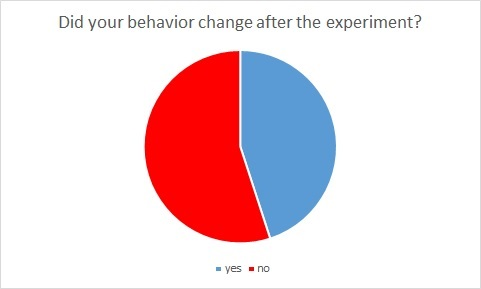
\includegraphics[width=1.0\columnwidth]{images/behavior_change.jpg}
\caption{\footnotesize Behavioural changes by participant group after the study \label{fig:behaviorchange} 
}
\end{figure}

    Most researchers hypothesize that often acknowledging and making these behaviors known lead to behavioral changes. Furthermore, it is believed that reflection upon a user's behavior also leads to changes. When asked if their behaviors changed after performing the experiment, those who said yes were asked to specify, and most of them state that they observed a certain behavior or noticed something new which led them to change their behavior which coincides exactly to what researchers found in the past. 
    The next question that should be asked is why people decided not to change their behavior after doing this experiment. For this set of data specifically, some of the information might shed light on why a little more than half of the participants decided not to change their behavior. There are three main reasons why we believe they might not have made behavioral changes:
    \subsection{No significant result found}
    For many participants, due to the short amount of time the experiment was run, many factors had effects on their experiment which contributed to the lack of statistical significance when attempting to prove their hypothesis. Therefore because their results were inconclusive, they have no reason to make changes to their behavior.
    \subsection{Hypothesis did not have clear cut good or bad behavior}
    For a couple of the participants, their hypothesis did not test a necessarily ‘bad’ behavior that they might want to change. For example, a participant tested whether apple vinegar affected their pH level. Another example is a participant who experimented with how much hot beverage she drank during the day depending on the temperature. These experiments don’t have a good or bad behavior associated with them and therefore does not call for behavioral change. 
    \subsection{No motivation to change}
    Finally, even if a participant found statistically significant results they might not believe that change is worth making other sacrifices. For experimental results to have an effect on a participant to elicit behavioral change, it must be significant to them. For example, one participants experiment asked what types of food affected him to the point of making them sick or greatly decreasing their mood. In this case it is of great value for the participant to change their behavior. On the contrary, if participants found significant results such as running increased sleep quality, perhaps running got in the way of more time of doing work or studying and so the participant believed that the opportunity cost of running for better sleep was not worth sacrificing time to do work. 

\section{Self Reporting}
Many students used self tracking in their experimentation. Different variables were tracked either using an app or a self-defined questionnaire. Mobile and desktop apps were used to track subjective variables such as mood. Apps with predefined scales for measuring variables were the preferred method of tracking subjective data. These apps sent scheduled reminders to track variables in the app, which helped many of the students consistently track the stages of their experiments. 

Several students created their own questionnaires to help them track their dependent variables. 
Participants felt that answering the same questions lessened the bias in their self reporting since they could record the same data in the same manner and do so with the same rating scale in mind. One participant came up with a series of questions and categorizations to classify the content and type of her dreams. Most of her questionnaire was very detailed and became less so towards the end of it. She mentioned that tracking her dreams might influence her answers later as she would get better at remembering her dreams and such, but that she tried to stay consistent in her ratings to have accurate data. Another self reported mood. He rated his mood three times a day (on waking, at noon, and before bed) on a scale of 1 - 5. 

Even though the students tried to lessen the bias of their self reporting, they felt that self reporting was the the most biased and error prone way to track in comparison to other devices and applications. A problem students had with self reporting was that other external factors would sometimes influence their ratings for mood, well-being, or tiredness and these events would not be catalogued, creating only a partial picture of what is really going on in their life. Participants noted these events may have influenced their results but felt they were integral to the study since they were studying themselves.

Even though the use of apps and devices appears to be the more mainstream and preferred way of tracking dependent variables, some types of data are too subjective to track automatically such as mood, tiredness and well being. These variables are best cataloged through self reporting. Some of our participants created their own method to accurately track the variables they were interested in to increase the accuracy of the data collected. Self reporting has tremendous potential in areas where apps cannot accurately gauge what kind of data users want to collect. It could also be useful for self trackers who are a lot older. Since this demographic of people typically do not use apps or modern technology, manual tracking could be a helpful way for these people to track their personal information. 

\section{User Background}
Within our class, we had representation from a relatively wide range of academic grade levels, from sophomores to PhD students, along with experience levels.  Upon gathering data from the members of the class via a survey sent out after the completion of the experiment, we were able to see how many member of the class had experience with statistics, took Jeff Huang’s undergraduate class Designing Developing and Evaluating User Interfaces (aka CS 1300), and who in the class had experimented with personal information tracking prior to conducting their experiment.  The information in the survey was given voluntarily and the students knew that their answers would not be anonymous.  While there are 21 students in the class, we only obtained 20 completed surveys and thus are omitting one person in the background examination of the experimenters. The composition of the class revealed by the survey results is shown in Fig.\ref{fig:surveybc}.  

\begin{figure}[!t]\centering
%\begin{wrapfigure}{o}{\textwidth}\centering
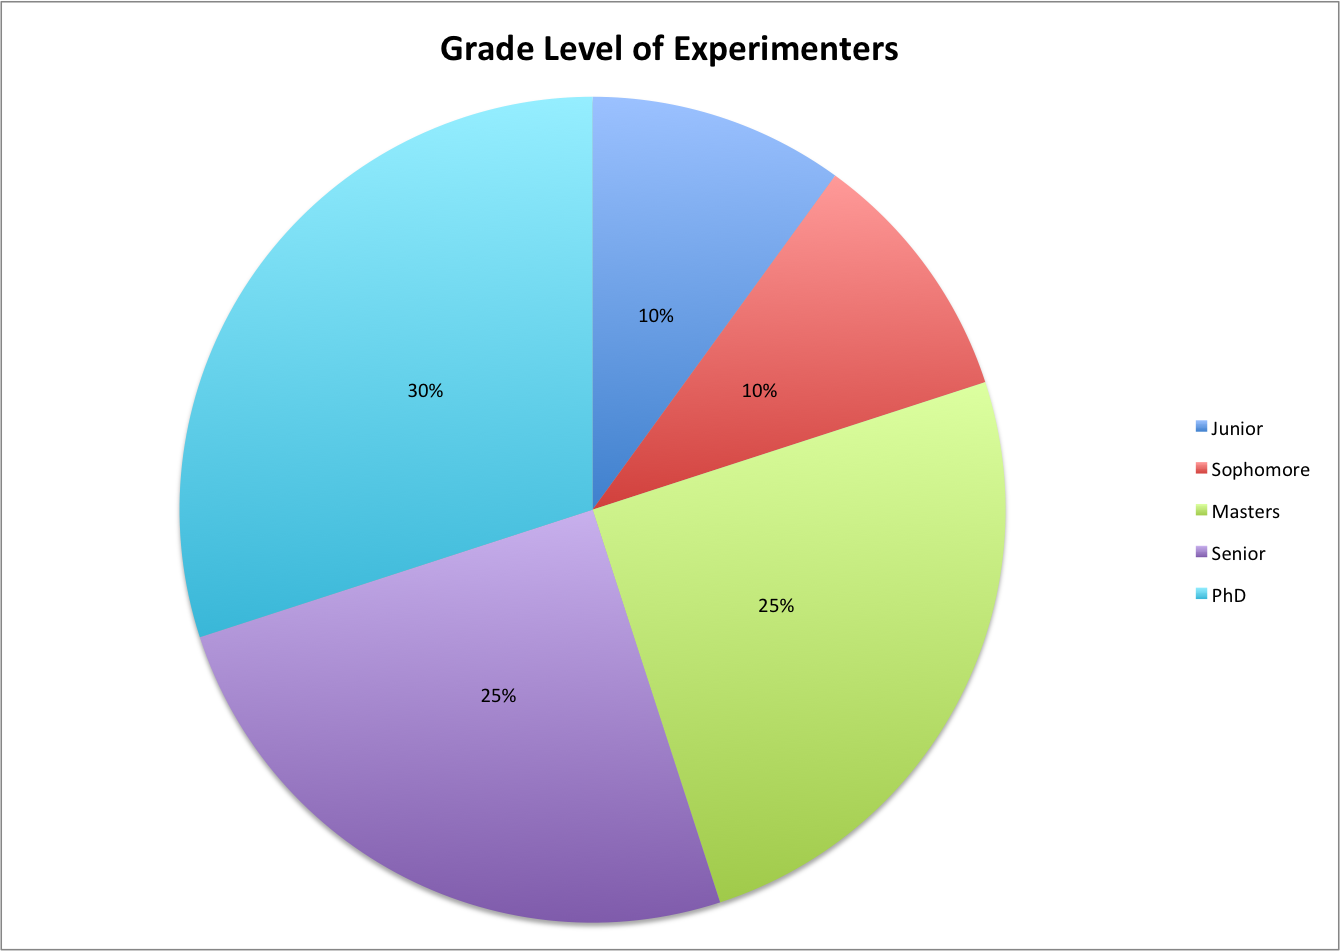
\includegraphics[width=1.0\columnwidth]{images/Grade_Level_of_Experimenters.png}
\caption{\footnotesize User Background in the class study \label{fig:surveybc} 
}%\end{wrapfigure}
\end{figure}

As can be seen above,  Masters, PhD and Senior students were all relatively equally represented while Juniors and Sophomore each only made up 10% of the class.  

In Fig.\ref{fig:table} is the experience levels of each of the twenty members of the class, broken down in combinations of experience levels. 

\begin{figure}[!t]\centering
%\begin{wrapfigure}{o}{\textwidth}\centering
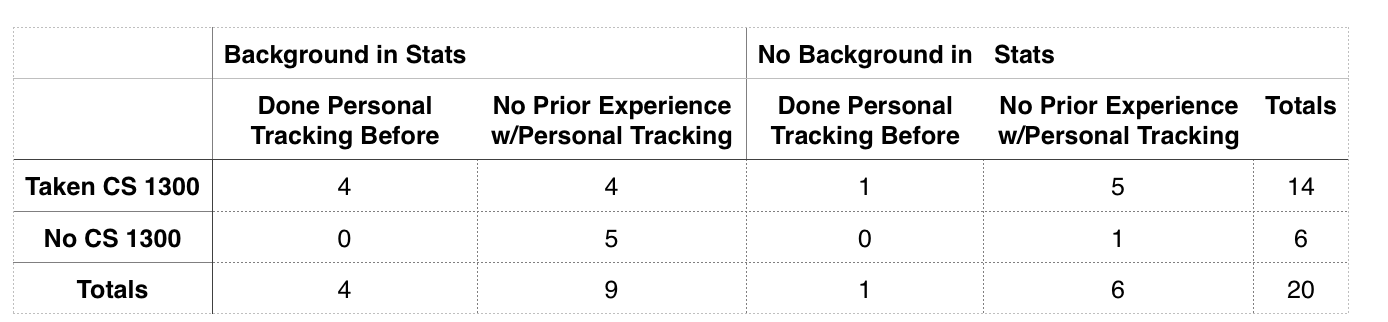
\includegraphics[width=1.0\columnwidth]{images/Backgrounds_of_Students.PNG}
\caption{\footnotesize Experience levels of participants \label{fig:table} 
}%\end{wrapfigure}
\end{figure}

There were many varying experience levels observed within the class.  While most students had either experience in statistics or taken Professor Huang’s undergraduate class prior to conducting their the experiments, there was a large number of observed combinations of the three types of experience we requested. The only combinations not observed were people who did not take CS 1300 but had done personal tracking before along with statistics and people who had not taken CS1300 and had no background in statistics but had done personal tracking.

\section{Methods of Analysis}
Between the 21 individual studies conducted, there were not only a large variety of dependent and independent variables tracked, but a wide variety of methods employed to analyze the data collected over the course of the experiment.  We tracked every pairwise combination of independent and dependent variables that the experimenters recorded and whose effects were analyzed.  In regards to the user created hypotheses, we also recorded whether each method of analysis supported the initial hypothesis, rejected the initial hypothesis, or was inconclusive.  The employed methods are shown in Fig.\ref{fig:analysis}

\begin{figure}[!t]\centering
%\begin{wrapfigure}{o}{\textwidth}\centering
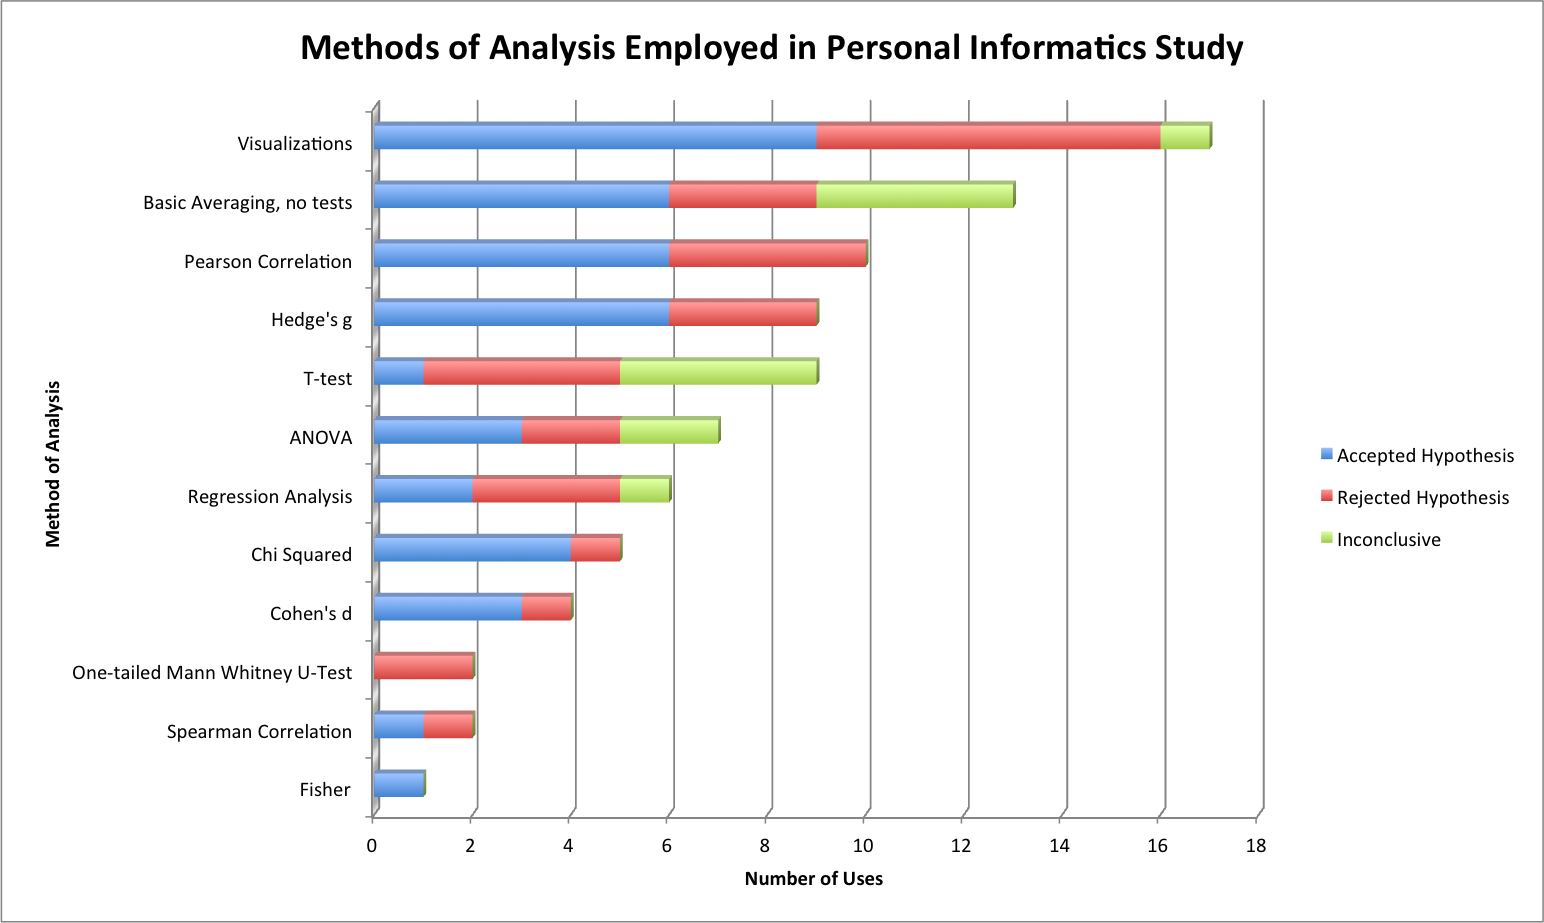
\includegraphics[width=1.0\columnwidth]{images/Methods_of_Analysis.png}
\caption{\footnotesize Employed methods of analysis \label{fig:analysis} 
}%\end{wrapfigure}
\end{figure}


Visualizations refers to the use of any graphs, plots, or other visual representations of the data collected and inferring relationships through mere observation.  This was the most popular method employed as many people used visualizations to accompany statistical tests they ran.  Of the visualizations, there was only one pairwise relationship whose effect, in regards to the user’s hypothesis, was deemed inconclusive.  Out of the 17 times these were used, 9 times the visualizations supported the hypotheses and 8 times they rejected the hypotheses.  While not all who used visualizations employed additional testing methods, given the test size of 1 and the relatively small time frame in which we conducted the experiments, it was considered acceptable to employ visualizations alone as a form of analysis. 

Basic averaging refers to the users who had to average some data points, usually per day or per session that they were tracking, and then comparing the average data.  This also required the use of no tests, however with dependent variables such as average heart rate throughout the duration of a work out, some users deemed this methods as the most appropriate way to gauge the existence or degree of an effect.  Of the 13 people who employed this method, 6 found their hypotheses to be supported, 3 found theirs to be rejected, and 4 found the data from averaging to be inconclusive.  In terms of variable such as heart rate, this may not have been the most effective way to see results.  Something such as average heart rate takes, usually, longer than 3-4 weeks to substantially change.  A better approach may have been to compare the high and low heart rates for each work, discarding the ascending and descending rate periods.  

Pearson’s correlation, or the correlation coefficient was used to measure the strength of the linear relationships between the independent and dependent variables.  Of the ten people to employ this method of analysis, there wasn’t a single person who found their results to be inconclusive.  This either supported the hypothesis, or rejected it.  This makes sense since there was no statistical test done on the actual correlation coefficient and so any correlation besides 0, which would be very unlikely to observe in scenarios such as these that are so dependent upon human behaviors, would render some sort of relationship. Out of these ten, 6 accepted and 4 rejected their hypotheses. 

As the fourth most common method of analysis employed, Hedge’s g also rendered no inconclusive results.  In terms of the effect size of independent variables on dependent variables, Hedge’s g had the same ratio that Pearson’s correlation did; 6 hypotheses were accepted and 4 were rejected.  As Hedge’s g reveals an effect and the size of that effect, it makes sense that hypotheses were either accepted or rejected, and that no one found their results to be inconclusive. 

While t-tests were the fifth most commonly used method of analysis, they were tied for the method that procured the most verdicts of inconclusive data.  Upon closer look, every user who employed a t-test used it to test the relationship between some dependent variable and either sleep quality or heart rate.  As both of these dependent variables are highly susceptible to a multitude of factors, all of which no one in the class recorded, it makes sense that those who used a t-test had the highest rate of finding their data inconclusive, as t-tests work best when there is large variance in the means of the data sets, a large sample size, and within the separate data sets, there is a low range, conditions not always applicable to heart rate and sleep quality, where in any given week there can be a wide range.  For individual experiments such as ours, a t-test may not have been the best method of analysis.

Seven pairwise relationships were tested using analysis of variance or ANOVA to gauge the effect of the dependent variable. This also had a proportionally high number of results rendered inconclusive to accept or reject the initial hypotheses. Of the seven, two were considered inconclusive, while two hypotheses were rejected and three were accepted. This makes sense as the basic ANOVA method generalizes a t-test to more than two sets.

As for the less common methods of analysis:
Regression analysis was used to test six hypotheses, two of which were accepted, three rejected and one accepted. 
Chi squared tests were used to test five hypotheses, four of which were accepted, and one rejected.
Cohen’s d was used to test the four hypotheses, three of which were accepted, one of which was rejected. 
A one-tailed Mann Whitney-U test was used for two hypotheses, both of which were rejected.
The Spearman Correlation was used for two hypotheses, one of which was accepted and one was rejected. 
Fisher’s exact test was used once, and it allowed the user to accept their hypothesis. 

From reading their reports and examining their respective findings, users seemed to have found drawing upon graphs and other visualizations very helpful in analyzing and then expressing their findings, in support of the statistical tests they ran.  In terms of small-scale studies such as ours, t-tests and ANOVA analysis seemed to procure a disproportionately large number of inconclusive verdicts, which we speculate is due to the small number of data points we collected, relative to larger, longer studies.

As far as detecting an actual effect and effect size, the testing methods that actually tested for size seemed to procure more definite results for our small scale testing, most prominently Hedge’s g. No doubt, as is later mentioned in our discussion, the varying backgrounds in statistics that were prevalent in our class affected the methods of analysis members employed.  The lesser used methods, such as the Spearman Correlation or Fisher’s exact test, are seldom taught, and not in depth, in introductory statistics classes, and thus those who had little background in or understanding of methods statistical analyses were at a disadvantage in terms of their methods of analysis. 

\section{Discussions on Error/Bias}

The focus of this study is to analyze how students might go about performing experiments in the department of personal informatics. Although the assignment specified various factors that users needed to take into account, it was vastly general and left the responsibility of design, decision, and analysis completely up to the user. This led to a wide range of different experiments and designs but often times users ran into similar problems.

%\begin{figure}[!t]\centering
%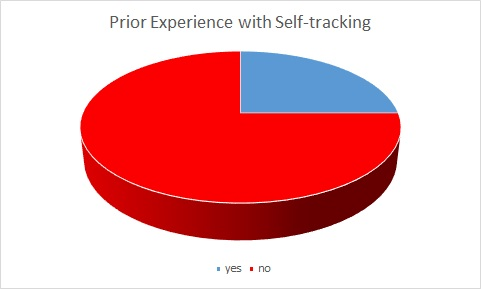
\includegraphics[width=1.0\columnwidth]{images/prior_experience.jpg}
%\caption{\footnotesize Prior experience of participants with self tracking \label{fig:experience} 
%}
%\end{figure}

In general, some participants had difficulty choosing the right design for their experiment. This includes those participants who would have benefited from using randomization rather than a variation of the AB design. Another error that various participants faced was a lack of statistical background and understanding which may have led to some naive conclusions in their report. Finally, an overall poor choice of variables to test was observed in many participants. When choosing a dependent variable, it should be something that is out of the user\textquotesingle s control, and therefore for students who chose sleep or productivity as their dependent variable, for example, because these variables are somewhat under their control (such as setting an alarm clock to wake up) these variables are not entirely dependent.  

Another concern for the majority of the participants of these studies were confounding factors that heavily affected their data. For example, the last week of the experiment happened to fall during spring break. As mentioned previously, most participants dealt with variables such as productivity and sleep, which for most is highly diminished and increased respectively during break. Other factors include participants who travelled or were sick during the experiment. These factors seemed to greatly impact the data for most participants.

Finally, most participants felt the study was too short and wished they could do it for longer, stating that 28 days was too little time to garner enough data points to have any statistically significance towards their hypothesis. Participants stated that due to the short time span, events such as exams, presentations, etc had bigger effects on their data than they would in the long run. 

\section{Areas of Improvements}

Some ways that this assignment might be improved in the future and yield better results might include some of the following:
\subsection{Running a longer experiment}
Running the experiment for a longer period of time would help eliminate the small outliers that had a great impact on the dataset due to the short amount of the experiment. This would also allow for less biases to be introduced depending on the amount of time. For example this could eliminate temporal biases such as seasons or other factors such as a big event etc. 
\subsection{Advice during design phase}
While participants read and discussed on the topic of personal informatics there was
little information about how and what decisions need to be made when planning an experiment design. Even when participants chose their variables there was little feedback on whether or not they would make for a good experiment. A higher degree of planning before starting the experiment might have even accounted for some of the confounding factors observed during the experiment. 
\subsection{Background in statistics}
    Although many students stated they had some background in statistics it would also be helpful to have had a lesson on what type of statistical tests to run on the different types of datasets and how to perform these correctly. A more structured run-through of how to do a N=1 experiment and how to run analysis would have benefited many of the participants. 

\section{Conclusion}
TODO


\section{Acknowledgments}


% Balancing columns in a ref list is a bit of a pain because you
% either use a hack like flushend or balance, or manually insert
% a column break.  http://www.tex.ac.uk/cgi-bin/texfaq2html?label=balance
% multicols doesn't work because we're already in two-column mode,
% and flushend isn't awesome, so I choose balance.  See this
% for more info: http://cs.brown.edu/system/software/latex/doc/balance.pdf
%
% Note that in a perfect world balance wants to be in the first
% column of the last page.
%
% If balance doesn't work for you, you can remove that and
% hard-code a column break into the bbl file right before you
% submit:
%
% http://stackoverflow.com/questions/2149854/how-to-manually-equalize-columns-
% in-an-ieee-paper-if-using-bibtex
%
% Or, just remove \balance and give up on balancing the last page.
%
\balance

\section{References format}
References must be the same font size as other body text.
% REFERENCES FORMAT
% References must be the same font size as other body text.

\bibliographystyle{acm-sigchi}
\bibliography{ref}
\end{document}
